\documentclass[11pt]{article}
\usepackage[margin=1in]{geometry}
\usepackage{amsmath,amssymb}
\usepackage{graphicx}
\usepackage{booktabs}
\usepackage{tikz}
\usepackage{hyperref}

\title{Typesetting at the Speed of Thought}
\author{The TexCraft Contributors}
\date{\today}

\begin{document}
\maketitle

\begin{abstract}
We describe a native editor that typesets as you type, keeps the source and the
PDF in step with SyncTeX, and is written entirely in Rust.
\end{abstract}

\section{Introduction}\label{sec:introduction}
Writing mathematics should feel like writing prose. Euler's identity
$e^{i\pi} + 1 = 0$ is a famous example, and the Gaussian integral
\[
  \int_{-\infty}^{\infty} e^{-x^2}\,dx = \sqrt{\pi}
\]
is another. Section~\ref{sec:method} explains the method.
% TODO: cite the original SyncTeX paper


\section{Method}\label{sec:method}
The heat equation on a rod of length $L$ is
\begin{equation}\label{eq:heat}
  \frac{\partial u}{\partial t} = \alpha \frac{\partial^2 u}{\partial x^2},
  \qquad 0 < x < L .
\end{equation}
Separating variables in Equation~\eqref{eq:heat} gives
\begin{align}
  u(x,t) &= \sum_{n=1}^{\infty} b_n \sin\!\left(\frac{n\pi x}{L}\right)
            e^{-\alpha (n\pi/L)^2 t}, \\
  b_n &= \frac{2}{L}\int_0^L f(x)\sin\!\left(\frac{n\pi x}{L}\right)dx .
\end{align}

\subsection{A picture}
% TODO: replace the sketch with measured data
\begin{figure}[htbp]
  \centering
  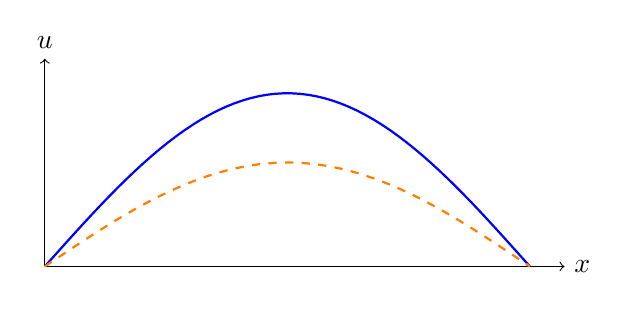
\begin{tikzpicture}[scale=1.1]
    \draw[->] (0,0) -- (6,0) node[right] {$x$};
    \draw[->] (0,0) -- (0,2.4) node[above] {$u$};
    \draw[thick, blue] plot[domain=0:5.6, samples=60] (\x, {2*sin(deg(\x*pi/5.6))});
    \draw[thick, orange, dashed] plot[domain=0:5.6, samples=60] (\x, {1.2*sin(deg(\x*pi/5.6))});
  \end{tikzpicture}
  \caption{Temperature profile at two times}\label{fig:profile}
\end{figure}

\subsection{Results}
\begin{table}[htbp]
  \centering
  \begin{tabular}{lrr}
    \toprule
    Engine & Cold start (s) & Live update (s) \\
    \midrule
    pdf\LaTeX & 0.61 & 0.38 \\
    Xe\LaTeX  & 1.42 & 0.95 \\
    Lua\LaTeX & 1.88 & 1.20 \\
    \bottomrule
  \end{tabular}
  \caption{Typesetting times for this paper}\label{tab:times}
\end{table}

Table~\ref{tab:times} and Figure~\ref{fig:profile} summarise the results; see
also \cite{knuth1984,lamport1994}.

Table~\ref{tab:times} and Figure~\ref{fig:profile} summarise the results; see
also \cite{knuth1984,lamport1994}.


\section{Conclusion}\label{sec:conclusion}
\begin{itemize}
  \item Live typesetting makes \LaTeX{} feel interactive.
  \item SyncTeX keeps the source and the output in step.
\end{itemize}

\bibliographystyle{plain}
\bibliography{refs}
\end{document}
